\chapter{Ameaças}\label{capitulo:ameacas}

As redes de computadores são alvos para inúmeras formas de ameaças. Será apresentado um conjunto compreendido por algumas das mais relevantes, levando em consideração sua capacidade de causar danos políticos, sociais e financeiros à sociedade, ainda que algumas delas tenham hoje em dia, somente sua importância histórica.

Antes de se atentar aos detalhes relacionados a tal seleção, é de grande valia que se saiba quais são os fatores que motivam os ataques, visto que são inúmeros os tipos de atacantes e alvos envolvidos no confronto.

Instituições de todos os gêneros e portes sofrem, frequentemente, com investidas advindas de diversos tipos de atacantes. Na maioria das vezes,  são acionadas ferramentas completamente automatizadas \cite{Botnets} e que não necessitam de interferência humana para cumprirem seus objetivos. Alternativamente, existem situações onde os ataques são direcionados, ou seja, são preparados e lançados por profissionais especializados em segurança e testes de penetração, sua bagagem técnina é grande, tendo envolvimento, em diversos níveis, com a comunidade \textit{Hacker}.

Pelo seu comportamento, pode-se atribuir aos atacantes diversas classificações, que variam de acordo com sua capacidade técnica e motivos que os levam à exploração de falhas, sendo que em muitos casos, chegam a praticar delitos em prol de benefícios individuais desejados.

As ameaças abordadas neste trabalho, podem ser visualizadas na tabela \ref{tabela:ameacas}, de acordo com sua classificação:

\begin{table}[H]
    \begin{center}
        \caption{\label{tabela:ameacas}Classificação dos tipos de ameaças}
        \begin{tabular}{c|p{8cm}}
            \hline
            \hline
                \textbf{Tipo de Ameaça} & \textbf{Classificação}\\
            \hline
                Cyber Warfare & Ameaça política\\
            \hline
                Redes de pedofilia & Ameaça social\\
            \hline
                Ataques de Negação de Serviço & Ameaça econômica e/ou política\\
            \hline
            \hline
        \end{tabular}
    \end{center}
\end{table}



\section{Cyber Warfare}

Historicamente, é comum que interesses de determinados grupos conduzam a humanidade a conflitos. Em geral, essas disputas envolvem diversos tipos de organizações, mediante os ideais que alimentam suas operações.

Nos dias de hoje, além dos conflitos armados entre as nações, são empregadas táticas de guerra nas redes de computadores, envolvendo grupos militares e paramilitares.

Em geral, as pessoas recrutadas para a participação neste tipo de atividade, recebem treinamento nas áreas de espionagem, segurança da informação, \textit{hacking} e \textit{Computação Forense}. Tais conhecimentos servem às organizações para espalhar caos e promover roubo de informações em instituições governamentais e privadas. Mesmo os governos e o setor privado, além de grupos criminosos, investem\cite{USCyberAttack} em capacitação do capital humano para que o fluxo de atividades relacionadas esteja sempre em alta.

Os ataques promovidos, vão além das fronteiras físicas e políticas, podendo afetar a todos que estejam conectados à \textit{Internet}. São alvos comuns: governos, instituições financeiras, grids científicos, \textit{ISPs}\sigla{ISP}{Internet Service Provider}, também conhecidos por \textit{Internet Access Providers} (\textit{IAP})\sigla{IAP}{Internet Access Provider} e até mesmo usuários domésticos. Existem casos mais críticos, onde o foco dos ataques são as redes de abastecimento de água e luz, infra-estruturas hospitalares, mecanismos de defesa militares e sistemas de robótica em organizações privadas.

É comum que grupos terroristas queiram desestabilizar governos, tentando promover possíveis quedas no abastecimento de serviços básicos, como foram constatados em ataques aos sistemas que controlam a rede elétrica norte-americana. No meio corporativo temos a espionagem industrial, ocorrida entre empresas concorrentes. Também fazem parte da lista, os crimes financeiros à bolsa de valores, que podem causar quebras de bancos e grandes empresas, endividamento de países inteiros e consequente diminuição do poder aquisitivo da população, como possível reflexo desse quadro.

O \textit{grid} de energia elétrica norte-americano, por exemplo, se conecta à várias redes, inclusive à \textit{Internet}, e tem grande parte de sua operação automatizada. Seu governo federal admitiu que o \textit{grid} é suscetível à guerra cibernética e levou a publico algumas notas onde são reportados ataques provenientes da China e Rússia\cite{ChinaWarfare} \cite{PragmaticJourneyWarefare} \cite{ChinhaRussianWarefare}. Um ataque com sucesso, neste caso seria o suficiente para interromper o fornecimento de energia elétrica para várias partes da nação, o que poderia causar desde traumas na opinião pública, abrir brechas para ataques militares distribuídos enquanto mantém pontos de distração perante à guarda, até um grande impacto econômico do país.

A promoção de guerras cibernéticas é, portanto, um forte indício de que se efetivaram inúmeras mudanças na maneira como a sociedade se reorganizou em torno da era da informação. Sem que sejam implantadas boas políticas de segurança e com o sucesso em ataques direcionados, pode-se ocasionar colapsos em inúmeros setores, básicos até mesmo para a manutenção da ordem em nações inteiras.


\section{Redes de pedofilia}

O fácil acesso à \textit{Internet}, trouxe às organizações criminosas espalhadas pelo mundo afora, a possibilidade da troca de informações de maneira ágil, no intuito de solidificarem e difundirem suas atividades ilícitas.

Atualmente, um dos grandes desafios dos profissionais de segurança, é auxiliar a justiça criminal no combate das redes de pedofilia, de modo que seja efetiva a perseguição aos infratores, devido seus agravantes contra a sociedade.

Uma prática comum entre este tipo de comunidade criminosa, é a busca por servidores comprometidos, que possam fornecer espaço em disco e banda suficiente para a hospedagem e distribuição de conteúdo multimídia, como fotos e vídeos, envolvendo suas vítimas. Tais criminosos podem utilizar canais de \textit{IRC} para comunicação instantânea, e hospedarem robôs especializados na distribuição de seus arquivos entre os interessados, de modo que os \textit{downloads} sejam redirecionados para servidores que eventualmente tenham sido tomados, para que a troca dos dados seja mais eficaz.

Existem também, redes de distribuição de pornografia infantil que comercializam seus materiais, mediante transações financeiras, que em sua grande maioria são internacionais, assim como evidencia um documento \cite{PESPORINT} produzido pelo Governo Brasileiro que, como colaboradores, teve diversos membros de organizações como a \textit{Associação Brasileira de Provedores de Serviços de Internet} (\textit{ABRANET}\sigla{ABRANET}{Associação Brasileira de Provedores de Serviços de Internet}) e a \textit{Agência Brasileira de Inteligência} (\textit{ABIN}\sigla{ABIN}{Agência Brasileira de Inteligência}), em conjunto com a \textit{International Criminal Police Organization} (\textit{INTERPOL}\sigla{INTERPOL}{International Criminal Police Organization}).

Por esta razão, é importante que sejam empregadas tecnologias que possam monitorar as atividades nas redes de computadores, principalmente em instituições cujo poderio computacional é grande. Dessa maneira, esta categoria de criminosos, poderá ser rastreada com mais facilidade por autoridades e \textit{Instituições de Pesquisa Forense Digital}, contribuindo em âmbito mundial, com a diminuição da quantidade de vítimas deste tipo de atividade ilegal.

\section{Ataques de Negação de Serviço em Rede}

Apesar de serem amplamente conhecidos, os ataques do tipo de Negação de Serviço \sigla{DoS}{Denial of Service} em Rede, também conhecidos pela terminologia inglesa \textit{Network Denial of Service} (\textit{NDoS})\sigla{NDoS}{Network Denial of Service}, são vistos a partir de diferentes óticas pela comunidade de pesquisadores e especialistas envolvidos em estudos de segurança. Não existe uma definição formal e genérica para estes tipos de ataques, pois cada um deles é fruto da observação de casos reais e da extração das técnicas empregadas em suas execução.\cite{NDoS}

Alguns autores os classificam como sendo tão somente o consumo, pelos atacantes, de recursos disponíveis na rede e que por consequência, fazem com que seu uso legítimo seja comprometido. Outros autores dizem que esses ataques têm a característica de causarem mau-funcionamento em dispositivos necessários para a entrega de pacotes, como é o caso de quando são disparados contra os \textit{roteadores}. Há ainda afirmações no sentido de que são fruto de qualquer ataque que resulte na indisponibilidade de informações, quando solicitadas, ou mesmo na corrupção destas. Todas essas abordagens mantém o foco no resultado gerado pelo ataque que, de uma maneira mais abrangente, resume-se na negação dos serviços solicitados.

Existem várias modalidades de ataques \textit{DoS}, dentre os quais, destacam-se por sua popularidade, importância histórica e caráter inovador, o \textit{Ping of Death}, \textit{Ping Flooding}, \textit{TCP SYN Flood} e \textit{DoS Distribuído}, sendo que a partir destes, surgiram ao longo do tempo, inúmeras variantes, cada uma com particularidades únicas, que as tornam efetivas nos ambientes para os quais foram projetadas. Seus principais aspectos técnicos serão abordados sequencialmente, de maneira que forneçam a este estudo uma visão mais ampla dos motivos pelos quais são consideradas tão destrutivos em ambientes interconectados em redes.


\subsection{Ping of Death}

Consiste em enviar \textit{pings} mal-formados (maliciosos), para um computador alvo. Um pacote \textit{ping} tem, por padrão, um tamanho de 56 \textit{bytes} (84 \textit{bytes}, se o cabeçalho for considerado) e historicamente, os Sistemas Operacionais não eram capazes de lidar com pacotes \textit{ping} que fossem maiores que o tamanho normal de um pacote \textit{IP}, o que corresponde a 65.535 \textit{bytes} \cite{RFC791}. Seria incorreto enviar um pacote maior que o tamanho máximo definido, mas é possível realizar isto se utilizando da capacidade de fragmentação dos pacotes.

Quando os sistemas operacionais recebiam pacotes fragmentados maiores que 65.535 \textit{bytes}, era frequente a ocorrência de comportamentos anormais, travamentos, e até mesmo \textit{reboots}, devido a um \textit{buffer overflow} que poderia ocorrer quando os pacotes maliciosos eram remontados. Esse exploit afetou muitos sistemas operacionais, como o \textit{Unix}, \textit{Linux}, \textit{Mac}, \textit{Windows} e até mesmo aqueles embarcados em impressoras e roteadores. No entanto, a grande maioria dos sistemas tiveram suas falhas corrigidas entre os anos de 1997 e 1998.

O problema em si não era relacionado ao protocolo utilizado pelo o utilitário \textit{ping} (\textit{ICMP}\sigla{ICMP}{Internet Control Message Protocol}, e sim ao processo de remontagem dos pacotes \textit{IP}, que podem carregar qualquer tipo de protocolo, como por exemplo \textit{TCP}\sigla{TCP}{Transmission Control Protocol}, \textit{UDP}\sigla{UDP}{User Datagram Protocol} ou \textit{IGMP}. O processo de correção desta falha consistiu em adicionar checagens durante a remontagem dos pacotes, onde para cada fragmento de pacote recebido, avalia-se os campos de \textit{deslocamento do fragmento} e \textit{comprimento total}, presentes em seu cabeçalho \textit{IP}, que somados não podem ultrapassar a marca de 65.535. Caso a soma seja maior, o pacote é invalidado e o fragmento \textit{IP} é ignorado. Tal checagem é realizada frequentemente em \textit{firewalls}, no intuito de proteger sistemas que não tenham essa correção implementada. Outra solução para este tipo de problema, embora não muito bem aceita por quebrar os padrões estabelecidos, é manter um \textit{buffer} maior que 65.535 \textit{bytes} para o processo de remontagem dos pacotes.

Atualmente outro tipo de ataque baseado em \textit{pings} é empregado, sua denominação é \textit{Ping Flood} e por definição, seu funcionamento é simples, baseando-se apenas na premissa de causar uma ``inundação'' de \textit{pings} no alvo, comprometendo a quantidade de tráfego na rede a qual este pode interagir. Isso faz com que o sistema vitimado tenha problemas tanto para responder às requisições realizadas, quanto para realizar novas requisições.



\subsection{Ping Flood}

Um ataque deste tipo, caracteriza-se por um \textit{DoS} onte o atacante sobrecarrega a vítima com pacotes \textit{ICMP Echo Request}. Sendo bem sucedido somente, se o atacante possui mais largura de banda disponível que a vítima (por exemplo, um atacante que possui um link \textit{DSL}\sigla{DSL}{Digital Subscriber Line} e uma vítima que possui um modem \textit{dial-up}). O atacante espera que a vítima responda com pacotes \textit{ICMP Echo Response}, consumindo toda sua banda de saída quanto sua banda de entrada.

Para reduzir os efeitos de uma inundação de \textit{pings}, pode-se utilizar \textit{firewalls} para ou filtrar completamente os pacotes \textit{ICMP Echo Request} de entrada, ou filtrar um grande número de requisições recebidas em um curto intervalo de tempo. Recusar a resposta produz dois benefícios: menos banda é desperdiçada quando não se responde às requisições e se dificulta ao atacante medir a efetividade de seu ataque. No entanto, tal atitude irá prevenir as medições de latência de usuários legítimos, o que pode ser indesejado, além de infringir as definições do \textit{RFC 1122}\sigla{RFC}{Request for Comment} \cite{RFC1122}. Uma solução mais elegante, consiste em filtrar somente os pacotes \textit{ICMP Echo Request} demasiadamente grandes ou então limitar a taxa com que o \textit{firewall} deixa passar os pacotes \textit{ICMP Echo Request}.

Não se pode confiar na procedência do endereço \textit{IP} remetente, uma vez que este pode ter sido falsificado, fazendo com que os pacotes \textit{ICMP Echo Request} pareçam vir de outros endereços, sejam eles específicos ou randômicos.


\subsection{Smurf attack}

Trata-se de um ataque \textit{DoS}, onde é gerada uma quantidade abusiva de tráfego na rede da vítima. A inundação ocorre com pacotes de \textit{ICMP Echo Response} e isso é possível pois, previamente, manipula-se maliciosamente os pacotes de \textit{ICMP Echo Request}, colocando-se o endereço \textit{IP} da vítima como remetente de todos os pacotes a serem enviados, que têm como destino vários endereços de \textit{broadcast} nas redes alcançáveis.

Se um dispositivo de roteamento, que entrega tráfego ao endereço de \textit{broadcast}, entregar como remetente dos pacotes \textit{ICMP Echo Request}, o mesmo endereço \textit{IP} de \textit{broadcast}, a maioria das máquinas nessa rede \textit{IP} responderão ao pacote recebido com um pacote \textit{ICMP Echo Response}, fazendo com que o tráfego seja multiplicado pelo número de máquinas que responderem. Em redes de \textit{broadcast} multi-acesso, isso faz com que centenas de máquinas possam responder a cada pacote.

Em meados de 1990, muitas redes \textit{IP} estiveram suscetíveis como alvos de ataques \textit{Smurf} (ou seja, responderem a \textit{pings} destinados a endereços de \textit{broadcast}). Devido à facilidade de se evitar este tipo de ataque e da conscientização da maioria dos administradores de rede, pouquíssimas redes se encontram vulneráveis nos dias de hoje.

Amplificadoras \textit{Smurfs}, são redes que se permitem utilizar, devido sua má-configuração, por ataques \textit{Smurf}. Em geral, agem amplificando o efeito deste tipo de ataque, pois geram quantidades enormes de pacotes \textit{ICMP Echo Response} aos alvos, através da falsificação de seus endereços \textit{IP}.

Para evitar o ataque, é preciso que sejam configurados, tanto roteadores quanto máquinas individuais, para que não respondam a \textit{pings} destinados a endereços de \textit{broadcast}. É preciso também, que se configure os roteadores para que não encaminhem pacotes diretamente a endereços \textit{broadcast}. Até 1999, os padrões adotavam como uma das características básicas dos roteadores, a capacidade de encaminhamento de pacotes para o endereço de \textit{broadcast}, o que foi abolido cerca de 1 ano mais tarde, mudando o os padrões da indústria e o comportamento dos roteadores, de modo que não mais encaminhassem esse tipo de pacotes.

Uma outra solução que pode ser empregada para evitar este ataque, é a chamada \textit{Filtragem de Entrada} aliada à \textit{Filtragem de Saída}, que irão avaliar quais são os endereços de \textit{IP} válidos, que são caracterizados pelas redes interconectadas fisicamente. Obviamente não é aplicável à \textit{Internet}, no entanto essa abordagem é extremamente pertinente quando utilizada entre \textit{ISPs}, Universidades e grandes corporações, devido ao fato de todos esses exemplos possuirem, em geral, várias redes internas interconectadas e também por se conectarem às redes externas de mesmo gênero, além da \textit{Internet}. Assim fica estabelecida uma ``política de boa vizinhança'' entre tais redes, onde só irão trafegar pacotes cuja fonte seja autorizada perante à topologia empregada.


\subsection{Fraggle Attack}

É um tipo de \textit{DoS}, em que o atacante envia uma grande quantidade de tráfego \textit{echo UDP} para endereços de \textit{broadcast}, todos com seus remetentes falsos. Trata-se de uma reescrita de código do ataque \textit{Smurf}. Ambos os ataques foram criados pelo mesmo autor, conhecido na comunidade por \textit{TFreak}. As portas alvo deste tipo de ataque são a 7 (\textit{echo}) e a 19 (\textit{chargen}).


\subsection{Christmas tree packet}

Um pacote \textit{Christmas tree} é determinado por possuir todas as opções possíveis para o protocolo que utiliza, marcadas como definidas. É também conhecido como pacote ``Kamizake'', \textit{nastygram} e \textit{lamp test segment}.

O termo deriva da analogia em que cada opção definida remete à lâmpadas com luzes com colorações diferenciadas umas das outras, frequentemente fixadas às árvores de Natal e, sendo todas estas opções ativadas, têm se um contexto onde todas as respectivas lâmpadas estariam acesas na árvore. Quando utilizados para \textit{scan}, as \textit{flags} definidas são \textit{FIN}, \textit{URG} e \textit{PSH}.

Pacotes \textit{Christmas tree} são utilizados como método de exploração da natureza da pilha \textit{TCP/IP}, através de seu envio e respectiva espera, ocorrendo assim uma análise das respostas obtidas. Muitos Sistemas Operacionais implementam seus próprios padrões para o protocolo \textit{IP} \cite{RFC791}, podendo apresentar implementações incompletas, de maneiras diferentes umas das outras. Pela observação de como um \textit{host} responde a um pacote inválido, como é o caso do \textit{Christmas tree}, pode-se tirar conclusões sobre o Sistema Operacional do alvo em questão. Versões do \textit{Microsoft Windows}, \textit{BSD/OS}, \textit{HP-UX}, \textit{Cisco IOS}, \textit{MVS}, e \textit{IRIX} mostram comportamentos que diferem do que é determinado pelo padrão estabelecido no \textit{RFC 791}, quando consultados sobre tais pacotes.

Alguns \textit{firewalls}, somente checam as políticas de segurança contra os pacotes que possuem a \textit{flag} \textit{SYN}\sigla{SYN}{Synchronize} definida, ou seja, que iniciaram a conexão de acordo com os padrões. Como os pacote \textit{Christmas tree} dedicados à atividades de \textit{scan} não possuem a flag \textit{SYN} definida, acabam furando estes sistemas de segurança e conseguem alcançar seus alvos.

Um número extenso de pacotes \textit{Christmas tree} podem inclusive, conduzir um ataque \textit{DoS}, aproveitando-se do fato de que tais pacotes exigem muito mais processamento por parte de roteadores e de seus alvos finais, em comparação com pacotes ``convencionais''.

Pressupondo-se que os pacotes \textit{Christmas tree} não são comumente encontrados nas redes (e tecnicamente, não seguem o padrão estabelecido pelo \textit{RFC 791} \cite{RFC791}), podem ser facilmente detectados por Sistemas de Detecção de Intrusões e \textit{firewalls} avançados. Da perspectiva de segurança nas redes, os pacotes \textit{Christmas tree} são sempre suspeitos e indicam uma alta probabilidade de que estejam sendo realizas atividades de reconhecimento na rede em questão.


\subsection{LAND}

Trata-se de um ataque muito disseminado em meados de 1997, explorava falhas na implementação do protocolo \textit{TCP/IP}, que na época, alguns Sistemas Operacionais e roteadores eram suscetíveis. Fora projetado inicialmente para afetar somente sistemas que rodassem \textit{Windows95}. \cite{TheLand}

Consistia bombardear o \textit{host} alvo com pacotes \textit{TCP} maliciosamente manipulados da seguinte maneira:

\begin{itemize}
    \item Definia-se a flag \textit{SYN} no pacote.
    \item As portas de entrada e saída eram definidas como sendo a mesma. No sistema para o qual foi projetado o ataque, era comum que se definisse uma das seguintes portas: \textit{113} ou \textit{139}, por fazerem parte das portas disponíveis em seu sistema de compartilhamento de arquivos em rede.
    \item Os endereços de \textit{IP} do remetente/destinatário eram definidos com o mesmo endereço do alvo.
\end{itemize}

O efeito obtido era o mal-funcionamento do sistema, pois teoricamente, este cenário não deveria existir sob condições normais. Como consequência de não possuirem um tratamento adequado para tal caso, os sistemas entravam em um estado instável o suficiente para que o único meio de se retomar as atividades, fosse através de um \textit{reboot} forçado nos computadores.

Com seu lançamento, esta falha trouxe à tona uma grande reviravolta nos meios de comunicação utilizados por profissionais de segurança e \textit{hackers}, em especial nos canais de \textit{IRC}, onde sempre foi comum a guerra entre os participantes, no intuito de se tomar o controle dos canais. Além disso, diversos fabricantes de roteadores e \textit{switches}, como a \textit{CISCO}, tiveram que tomar medidas par readequadar em seus produtos, no intuito de suprimir tal falha com sucesso. \cite{LandExperiences}


\subsection{SYN flood}

% Adaptação livre dos textos retirados de \textit{RFC 4987 TCP SYN Flooding Attacks and Common Mitigations} e \textit{http://www.iss.net/security\_center/advice/Exploits/TCP/SYN\_flood/default.htm}

Quando um cliente tenta iniciar uma conexão com um servidor, ambos trocam uma série de mensagens, descritas normalmente como:

\begin{enumerate}
    \item O cliente requisita uma conexão enviando uma mensagem \textit{SYN} (\textit{sinchronize}) para o servidor.

    \item O servidor reconhece a requisição, enviando uma mensagem \textit{SYN-ACK}\sigla{SYN-ACK}{Sinchronize-Aknowledge} (\textit{sinchronize-aknowledge}) de volta para o cliente.

    \item O cliente responde com uma mensagem \textit{ACK}\sigla{ACK}{Aknowledge} (\textit{acknowledge}) e então, a conexão é estabelecida.
\end{enumerate}

Este processo é chamado de \textit{TCP three-way handshake}, sendo a base para toda conexão estabelecida ao se utilizar o protocolo \textit{TCP}. A figura \ref{figura:threeway} mostra o funcionamento do processo descrito:

\begin{figure}[H]
    \begin{center}
        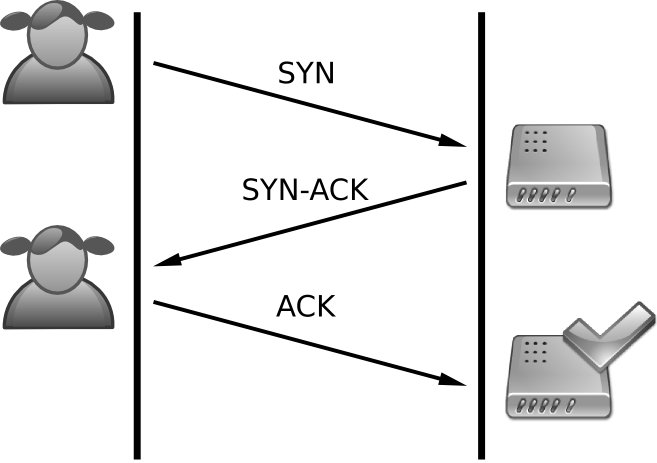
\includegraphics[scale=0.6]{./figuras/Tcp_normal-GS.png}

        \caption{\label{figura:threeway}Usuário legítimo, se conectando ao servidor utilizando o \textit{three-way-handshake}.}
    \end{center}
\end{figure}

O \textit{SYN flood} é um ataque bem conhecido e geralmente, não é efetivo contra redes modernas. Seu funcionamento depende do servidor alocar recursos depois do recebimento de um \textit{SYN} e adicionalmente, antes que receba o \textit{ACK}.

Existem dois métodos de ataque, ambos consistindo na premissa de que o servidor não receba o \textit{ACK}:
\begin{itemize}
    \item Um cliente malicioso pode evitar o envio do último \textit{ACK}, fazendo com que o servidor fique sempre esperando pelo mesmo e tenha os recursos alocados comprometidos.

    \item O endereço de \textit{IP} que originou o \textit{SYN} enviado pode ser falsificado, fazendo com que o servidor envie o \textit{SYN-ACK} para um \textit{IP} falso, não recebendo então, o último \textit{ACK}.
\end{itemize}

Em ambos os casos, o servidor irá esperar pelo último \textit{ACK} durante algum tempo, tendo como efeito o mesmo que uma congestão na rede, de modo que este \textit{ACK} restante não seja recebido no tempo certo. A figura \ref{figura:threeway_synflood} mostra o funcionamento do processo descrito:

\begin{figure}[H]
    \begin{center}
        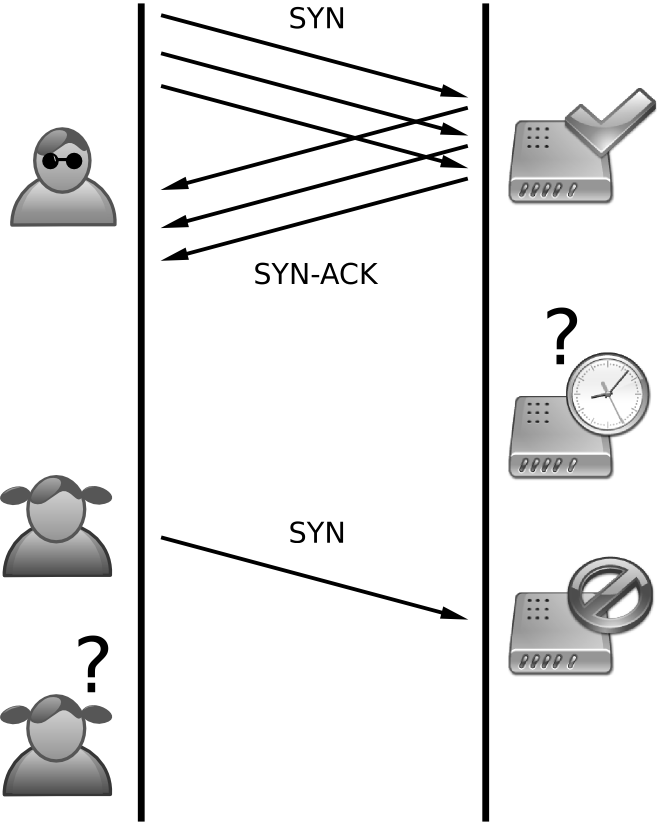
\includegraphics[scale=0.6]{./figuras/Tcp_synflood-GS.png}

        \caption{\label{figura:threeway_synflood}Ataque \textit{SYN flood} é lançado, efetivando o \textit{DoS}.}
    \end{center}
\end{figure}

Se estas conexões incompletas ocuparem recursos no servidor, pode ser possível tomar todos os recursos disponíveis através de uma inundação de requisições \textit{SYN}, daí sua definição. Uma vez que todos os recursos sejam reservados por estas conexões incompletas, sejam elas legítimas ou não, o resultado obtido é a negação de serviço para os demais clientes. Alguns sistemas podem falhar, através de um mal-funcionamento ocasionado por sua arquitetura, ou mesmo travarem, caso alguns recursos do Sistema Operacional estiverem correlacionados aos recursos que foram consumidos com o ataque.

Em meados de 1996, era comum a alocação de recursos para conexões incompletas \textit{TCP}, através da utilização de uma fila, que era em geral, bastante curta, contando com aproximadamente 8 entradas, onde cada uma destas entradas era removida somente quando a conexão era completada ou então, quando expirava seu tempo de vida, que era de aproximadamente 3 minutos. Quando essa fila estava cheia, futuras conexões falhariam, sendo uma tarefa fácil a de comprometer sistemas com este caráter, pois com apenas 8 pacotes enviados em sequência num intervalo de 3 minutos para cada uma, era possível se atingir uma negação de serviço dispondo do mínimo de recursos.

O \textit{SYN flood} explora esse caráter falho na arquitetura das conexões \textit{TCP} e por isso, para mitigar os riscos existem técnicas que fogem do domínio do protocolo, sendo apenas formas parciais de defesa, que devem ser utilizadas em conjunto para que sejam efetivas. Para que isso seja possível, pode-se empregar as seguintes abordagens:
\begin{itemize}
     \item \textit{SYN cookies}: O envio do \textit{SYN-ACK} é realizado com números sequenciais cuidadosamente construídos, contendo um \textit{hash} criptográfico, gerado a partir de informações tais como o endereço \textit{IP} do cliente e o número da porta utilizada pela conexão. Quando o cliente responder com um \textit{ACK} normal, essa sequência será inclusa no pacote, que será comparada pelo servidor, no intuito de verificar a autenticidade do mesmo. Adicionalmente, a alocação de memória é realizada pelo servidor durante o envio do terceiro pacote do \textit{three-way-handshake}, e não durante o recebimento do primeiro pacote.

    \item \textit{RST cookies}\sigla{RST}{Reset}: É um método alternativo à utilização dos \textit{SYN cookies}, onde o servidor envia aos clientes um \textit{SYN-ACK} que contenha erros em sua descrição, desta maneira, se o cliente for autêntico, enviará uma mensagem de \textit{RST} ao servidor, que verificará sua autenticidade, não tendo seu endereço \textit{IP} considerado como falso, então o processo de \textit{three-way-handshake} pode se repetir de maneira correta e a conexão é estabelecida com sucesso. Pode causar problemas com máquinas que utilizem o Sistema Operacional \textit{Windows95} ou que estejam protegidas por \textit{firewalls}. Pelo segundo motivo, não é uma técnica amplamente adotada pela comunidade.

    \item Alocação de micro-blocos: Consiste em não alocar registros completos para cada conexão, sendo que implementações modernas realizam a alocação de apenas 16 \textit{bytes} como forma de prevenção do esgotamento de recursos de memória.

    \item Modificações na pilha \textit{TCP/IP}: Reduz os riscos do \textit{SYN flood}, através da redução do tempo limite de expiração dos registros alocados no início do \textit{three-way-handshake}. Uma abordagem comum envolve modificações baseadas em algoritmos que seletivamente descartam conexões de entrada específicas.
\end{itemize}


\subsection{Stacheldraht}

Traduzindo-se do alemão, significa ``arame farpado''. Foi escrito por \textit{Random} e ganhou popularidade no verão norte-americano de 1999. Trata-se de um agente que atua em ataques \textit{DoS} distribuídos, ou \textit{DDoS}\sigla{DDoS}{Distributed Denial of Service}. Afeta sistemas \textit{Linux} e \textit{Solaris}, sendo capaz de realizar falsificações nos endereços \textit{IP}. Utiliza outros ataques \textit{DoS}, como: \textit{UDP flood}, \textit{ICMP flood}, \textit{TCP SYN flood} e \textit{Smurf attack}. Notavelmente, combina as redes \textit{Trinoo} e \textit{TFN}\sigla{TFN}{Tribe Flood Network} em seus ataques \textit{DoS distribuídos}. Utiliza criptografia na comunicação entre atacante e ``máquinas-escravas'', além de possuir atualizações automáticas de seus agentes.

Ao analisar sua arquitetura \cite{Stacheldraht}, nota-se que um atacante pode se conectar a vários gerenciadores intermediários. Cada gerenciador é capaz de controlar no máximo 1000 máquinas comprometidas, que por sua vez, irão receber ordens através de um canal seguro de comunicações. Existe um terminal interativo entre atacante e gerenciador, que se assemelha a um terminal de \textit{telnet}, com opções que permitem o controle total do ataque, oferecendo meios para a adição de novos endereços \textit{IP} de vítimas, iniciar ataques, parar ataques, verificar quais estações estão \textit{offline}, entre outras. Para que seja possível o acesso ao terminal dos gerenciadores, uma senha é requisitada ao atacante, que por padrão é denominada ``sicken''. Essa característica foi determinada através de engenharia reversa. Seu método de criptografia utilizado para o armazenamento da senha é o \textit{crypt()}, muito conhecido nos sistemas \textit{UNIX}, que posteriormente é submetido ao método de cifragem simétrica \textit{Blowfish}, cuja palavra-chave é ``authentication'', assim como também o são, todas as mensagens que são trocadas na comunicação cliente/servidor.

Assim como se faz com o \textit{Trinoo} e com o \textit{TFN}, o método de instalação é o mesmo que em qualquer sistema \textit{UNIX} comprometido, com opções para que se possa esconder arquivos e programas (por exemplo, diretórios ocultos e \textit{rootkits}). Uma característica que não é presente nem no \textit{Trinoo} e nem no \textit{TFN}, é sua auto-atualização, que se dá através do comando ``rpc'' da família \textit{Berkeley} (porta \textit{514 TCP}), utilizando contas roubadas em servidores comprometidos. Então, todos os agentes e controladores são instruídos a buscarem versões mais recentes de si mesmos e substituirem suas versões antigas pelas mais novas que por ventura sejam obtidas.

Seu conjunto de ferramentas utiliza extensivamente pacotes \textit{ICMP Echo Reply}, sendo assim, uma tarefa muito difícil consiguir bloquear seu funcionamento sem que os outros serviços de rede baseados nessa mesma tecnologia não sejam comprometidos. Em grandes redes é impraticável que se realize uma análise de pacotes \textit{ICMP Echo Request} e \textit{ICMP Echo Reply}, afim de se distinguir tráfego legítimo (como o do utilitário \textit{ping}) do tráfego malicioso.


\subsection{UDP flood attack}

\textit{UDP} é um protocolo que não requer que sejam mantidas conexões e não necessita que seja estabelecido um processo de inicialização para que as conexões ocorram. O \textit{UDP Flood Attack} é um tipo de ataque \textit{DoS}, onde o atacante envia pacotes \textit{UDP} para portas aleatórias no sistema vitimado. Quando esse sistema recebe o pacote \textit{UDP}, irá determinar que aplicação está a sua espera na porta informada. No momento que interpreta os dados e conclui que não existe tal aplicação esperando pelos dados, irá gerar um pacote \textit{\textit{ICMP} marcado como Destination Unrechacle}, que será enviado para o \textit{host} cujos dados partiram, sendo este classificado como seu remetente. Se forem enviados pacotes \textit{UDP} em uma quantidade suficiente para alvo, e estes forem entregues com sucesso nas portas especificadas, o sistema poderá sofrer uma queda.

Para que o \textit{UDP Flood Attack} seja efetivamente reduzido, deve-se implantar \textit{firewalls} em localizações críticas da rede, no intuito de filtrar os dados indesejados e provenientes de remetentes falsos. Adicionalmente, as ações seguintes podem ser tomadas:
\begin{itemize}
    \item Desabilitar e filtrar os serviços \textit{chargen} e \textit{echo}, assim como os demais que funcionem com \textit{UDP} e que não sejam utilizados.

    \item Utilização de \textit{proxys} para prover serviços \textit{UDP} que sejam essenciais, no intuito de serem protegidos contra o mal-uso.

    \item Monitorar a rede, para identificar os usuários do serviço, assim como o possíveis abusos.
\end{itemize}




\section{Malwares}

% Adaptação livre do texto retirado do endereço \textit{http://www.linfo.org/malware.html}.

\textit{Malwares} são definidos como qualquer software desenvolvido com propósito de causar dandos aos computadores, ou de utilizá-los como meio de realizar atividades ilegais. Podem ser classificados de várias maneiras, incluindo como parâmetro, o princípio utilizado para que sejam disseminados, como são executados e/ou as atividades que realizam. Os principais tipos de \textit{malwares} incluem \textit{worms}, \textit{vírus}, \textit{trojans}, \textit{backdoors}, \textit{spywares}, \textit{rootkits} e \textit{spams}.

\textit{Worms} e \textit{vírus}, são programas de computador que se replicam se a intervenção humana. A diferença básica entre ambos, é que os \textit{vírus} se anexam aos executáveis, tornando-se parte dos mesmos, enquanto que os \textit{worms} são auto-suficientes, não precisando se tornar parte de outro programa para que se repliquem. Adicionalmente, enquanto os \textit{vírus} são projetados para causar problemas no sistema local e são passados através de setores de \textit{boot} dos discos, anexos em \textit{E-Mails} ou mídias removíveis, os \textit{worms} são projetados para explorar o ambiente conectado em rede. Uma vez executado, um \textit{worm} busca ativamente por outros computadores suscetíveis às mesmas falhas às que fora projetado para explorar, ao contrário dos \textit{vírus}, que são programados para buscar por partes específicas do sistema local, mas que sejam vulneráveis à infecção, onde se replicam e mantém o máximo controle que puderem sobre sua execução.

\textit{Trojans}, ou cavalos de tróia, são \textit{softwares} distribuidos como sendo supostamente legítimos, com o objetivo de incitar os usuários a fazerem o \textit{download} dos mesmos e instalá-los em seus sistemas. Em contraste com os \textit{worms} e \textit{vírus}, os \textit{trojans} não são diretamente auto-replicáveis. São projetados para realizarem atividades perigosas, incluindo a corrupção de arquivos (muitas vezes de maneiras subitas), apagar dados e instalar outros tipos de \textit{malwares}.

\textit{Backdoors} são programas que fornecem acesso remoto aos sistemas de maneira infiltrada e escondida. Trabalham tipicamente permitindo que indivíduos ou mesmo outros sistemas, que saibam de sua presença, utilizem senhas especiais e/ou ações específicas que passem pelos métodos comuns de autenticação presentes em máquinas remotas, no intuito de obterem acesso especial às contas administrativas. São projetados para se manterem escondidos, mesmo com inspeções cuidadosamente realizadas.

\textit{Spywares} são \textit{softwares} que são instalados nos computadores com o propósito de obterem informações sobre o mesmo, incluindo seus usuários e/ou outros computadores conectados na mesma rede aos quais as máquinas hospedeiras se comunicam. Os tipos de informação obtidas, em geral são nomes de usuários e suas senhas, hábitos de navegação na \textit{Internet}, dados financeiros como contas bancárias e cartões de crédito, ou transações secretas. Uma aplicação comum dos \textit{spywares} é mostrar \textit{popups} por meio dos \textit{browsers} utilizados pelos usuários, com base em seus hábitos de navegação na \textit{Web}.

\textit{Rootkits} são programas secretamente inseridos em computadores, que permitem que os intrusos ganhem acesso à contas administrativas dos sistemas, sendo assim capazes de controlar todos os aspectos dos computadores. Incluem, frequentemente, funções para que seus traços sejam escondidos depois de penetrarem no sistema, através da remoção dos arquivos de \textit{log}, por exemplo. Tipicamente incluem \textit{backdoors}, permitindo que o intruso obtenha posteriormente, acesso facilitado aos sistemas em questão, para que possa efetuar ataques em datas específicas.

\textit{Spam} é um tipo de \textit{E-Mail} indesejado, enviado em larga escala para os usuários. Apesar das pessoas receberem poucos \textit{spams} por dia e sua grande maioria acabar sendo barrado por sistemas \textit{anti-spam}, pode-se imaginar que este tipo de inconveniente não seja um grande problema a ser tratado. No entando, para os responsáveis pela manutenção da infra-estrutura que hospeda os serviços de \textit{E-Mail}, este é um sério agravante, pois gera um grande volume de dados a serem armazenados, correspondendo, em geral, a mais da metade de todos os \textit{E-Mails} autênticos armazenados, o que ocasiona uma grande carga nos sistemas responsáveis pelo gerenciamento dos mesmos. É comum que contenham certos tipos de \textit{malwares} e que muito de seu conteúdo seja utilizado para efetivar fraudes. As organizações do mundo todo dedicam recursos consideráveis nas tarefas de filtragem e remoção dos \textit{E-Mails} considerados \textit{spam}, tomando os devidos cuidados para que não comprometam \textit{E-Mails} legítimos de sua base de usuários.

Existem várias razões básicas pelas quais os \textit{malwares} são criados. São empregados sentimentos de concretização de metas, desejo de mostrar capacidades técnicas, vontades que impulsionam a causar danos ou motivos financeiros. Este último, é provavelmente o mais importante de todos, pois existem grandes incentivos financeiros para que tais atividades sejam desenvolvidas, principalmente de/para organizações criminosas e em menor grau, a indivíduos especialistas em segurança de computadores, contratados para assistirem o desenvolvimento dos mesmos.

O prejuízo causado pelos \textit{malwares} pode ser muito grande. Por exemplo, pode levar à indisponibilidade de computadores e redes inteiras, até que sejam reparados, o que pode ocasionar altos custos financeiros para seus responsáveis. Podem resultar na corrupção ou roubo de dados confidenciais, assim como no roubo de fundos. Adicionalmente, podem resultar em perdas temporárias e/ou danificação de equipamentos que dependem de computadores, que por ventura sejam vitimados.

Danos similares podem resultar advindos de \textit{softwares} que sejam mal-projetados/escritos que, assim como os malwares, têm presença muito comum em meio às organizações. No entanto, a distinção entre ambos é dada subtamente. Enquanto os \textit{malwares} são criados inteiramente, ou principalmente, no intuito de causarem injúrias ou beneficiarem seus criadores, às custas de outros indivíduos, os danos são consequência secundária no caso de \textit{softwares} defeituosos, pois estes raramente são seu motivo de existir.

Existem inúmeros passos que os usuários de computadores podem tomar para que as chances de se infectarem por \textit{malwares} sejam minimizadas. São incluidas como boas práticas, a utilização de \textit{softwares} legítimos e seguros, a provisão de locais físicos que sejam seguros aos computadores e às redes, a adoção de políticas obrigatórias na definição de senhas seguras, implantação de \textit{firewalls}, utilização de programas de detecção de \textit{malwares}, evitar abrir \textit{E-Mails} com anexos cujos remetentes sejam desconhecidos, evitar o \textit{download} de programas dúbios e evitar o uso de contas administrativas para tarefas corriqueiras, sendo que  estas devem ser utilizadas somente quando necessário.

Alguns tipos de Sistemas Operacionais e aplicações são muito mais resistentes aos \textit{malwares} que outros, particularmente aqueles baseados no \textit{Kernel} do \textit{Linux} e outros Sistemas Operacionais \textit{Unix-like}. Esse fato se deve por terem sido projetados para evoluir ao longo do tempo, levando-se em consideração a segurança como fator essencial, ao invés de tomar uma abordagem na qual as tentativas de se adicionar camadas de segurança fossem implantadas posteriormente.

Também deve-se levar atentar ao fato de que são raras as tentativas de se projetar \textit{malwares} para esses sistemas. Uma razão que justifica isso é que o número de computadores que os utiliza, ainda é a minoria, ocasionando em um menor número possíveis alvos para os criminosos, sendo menos interessante desprender esforços para atingir sua gama de usuários. O fato de serem melhor projetados quanto os requisitos de segurança, dificulta a produção de \textit{malwares} que sejam eficientes e bem sucedidos nas investidas de ataque.

Devido sua importância, os \textit{malwares} merecem um estudo minucioso, além do estabelecimento de sistemas capazes de detectar novas variantes destes, já que a manutenção do bom funcionamento dos computadores e de suas redes, é de suma importância para todas as organizações do mundo.
